\documentclass[12pt]{beamer}
\usepackage{beamerthemeHannover, graphicx, clrscode, amsmath, amssymb, multicol}
\usepackage{verbatim}
\setbeamercolor{sidebar}{use=structure,bg=gray!60!green}
\title{Introduction To Perl 6 Modules}
\author[Duke Leto]{Jonathan "Duke" Leto}
\date{}

\begin{document}

\frame{
    \titlepage
    \begin{center}
        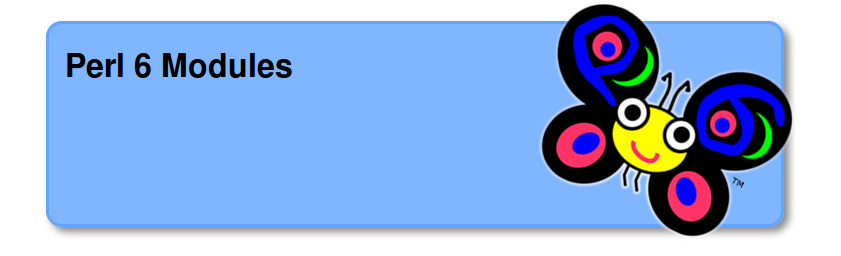
\includegraphics[scale=0.3]{perl6modules}
    \end{center}
}

\frame{
    \frametitle{What is Perl 6?}
    \begin{center}

    \begin{itemize}
        \item It is a specification for a language.
        \item There are many implementations.
        \item NOT the successor to Perl 5 (more like a kid sister).
    \end{itemize}
    \end{center}
}

\frame{
    \frametitle{What are Perl 6 Modules?}
    \begin{center}

    \begin{itemize}
        \item Just like Perl 5 modules, Perl 6 modules are units of distributable and
        useful code.

        \item The CPAN of Perl 6 is called http://modules.perl6.org
        \item How many modules does your unreleased language have?
    \end{itemize}
    \end{center}
}

\frame{
    \frametitle{Which flavor of Perl 6?}
    \begin{center}
    \begin{itemize}
        \item Different flavors of Perl 6 have implemented different feature sets.

        \item Rakudo Perl 6 currently has the largest feature set and the most number of current contributors.
        \item Most Perl 6 modules worked on Rakudo at least some time in the past.
    \end{itemize}
    \end{center}
}

\frame{
    \frametitle{Anatomy of a Perl 6 Module}
    \begin{center}
    \begin{itemize}
        \item It looks just about the same!
        \item META.info (like a Build.PL or Makefile.PL)
        \item README*
        \item lib/
        \item t/
    \end{itemize}
    \end{center}
}

\frame{
    \frametitle{What does META.info look like?}

    It is just a chunk of JSON with project metadata.

    \begin{center}
        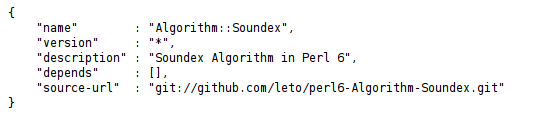
\includegraphics[scale=0.5]{soundex_meta_info}
    \end{center}

}

\section{How Do I Install a Perl 6 Module}

\frame{
    \frametitle{How Do I Install a Perl 6 Module}

    You must enlist the help of a panda!

    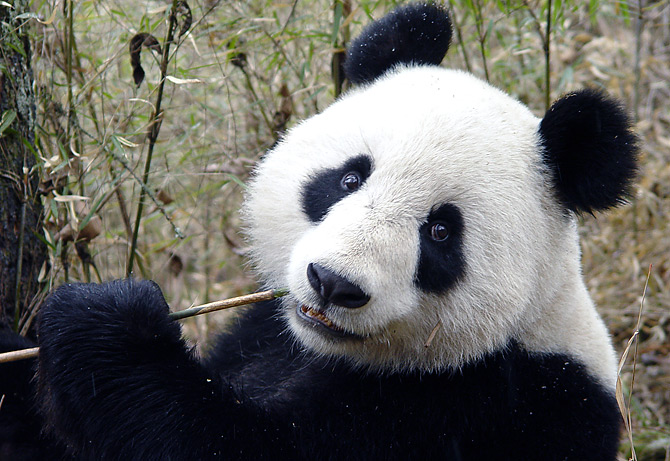
\includegraphics[scale=0.3]{panda1}
}

\frame{
    \frametitle{Installing Panda}

    First, we grab panda (the cpanminus of Perl 6):

    \begin{itemize}
    \item git clone git://github.com/tadzik/panda.git
    \item cd panda
    \item sh bootstrap.sh \# needs a perl6 binary in PATH
    \end{itemize}
}

\frame{
    \frametitle{Installing a Perl 6 Module with Panda}
    So simple, even your grandma could do it:
    \begin{itemize}
    \item panda install Algorithm::Soundex
    \end{itemize}
}

\section{How Do I Write A Perl 6 Module?}
\frame{
    \frametitle{How Do I Start Writing a Perl 6 Module?}

    \begin{itemize}
    \item git clone https://github.com/tadzik/module-starter
    \item cd module-starter
    \item module-starter --description="some junk" Some::Junk

    \end{itemize}
    Now you have directory Some-Junk/ with a META.info!
}

\frame{
    \frametitle{Show me the code!}



\frame{
    \frametitle{Writing Tests for a Perl 6 Module}
}

\frame{
    \frametitle{Running Tests for a Perl 6 Module}
}

\section{Getting Started}
\frame{
    \frametitle{Getting Involved}
}

\section{ Let's Jump In }
\frame{
    \frametitle{Hack Session}
    Ok, let's do some hacking already.
    \begin{itemize}
        \item Checkout source code (git clone ...)
        \item Build Rakudo
        \item Run the Perl 6 Test Suite (long but fun!)
        \item Submit bugs if any tests fail
        \item Experiment!
    \end{itemize}
}

\frame{
    \frametitle{ Thanks }
    \begin{itemize}
        \item Larry
        \item Eric Wilhelm
        \item Patrick Michaud
        \item The Perl Foundation
        \item Everyone working on Parrot, Rakudo and Perl 6
        \item PDX.pm for listening to my rants
    \end{itemize}
}

\frame{
    \frametitle{ Resources }
    \begin{center}
        \begin{itemize}
           \item http://perl6.org
           \item http://modules.perl6.org
           \item TODO: perl 6 planet
           \item \#perl6 on irc.freenode.net
           \item \#parrot on irc.perl.org
        \end{itemize}
    \end{center}
}
\end{document}
